\section{The modular group and continued fractions}

For an arbitrary modular transformation $A$, a representation as product of shifts $U^j: z \mapsto z+j$ and inversions $T: z \mapsto -\reci{z}$ can be found by the algorithm described in Corollary \ref{cor_ModGrpTUAlg}. By writing out this product, for example in the case when $n=2$, we have
\begin{equation*}
A = U^{e_0}T U^{e_1}T U^{e_2}T U^k,
\end{equation*}
or more explicitly
\begin{equation}
\label{eqn_ALongConFrac}
A(z) = e_0 - \reci{e_1 - \reci{e_2 - \reci{k + z}}}.
\end{equation}
\index{Continued fraction}
\index{Pringsheim notation}
Here a close relation between modular transformations and continued fractions immediately gets apparent. In this section we will investigate this relation somewhat deeper. 
First we will use Pringsheim's more space-saving notation for continued fractions, namely
\begin{equation}
\label{eqn_ConFracNotation}
b_0 + \frac{a_1}{b_1 + \frac{a_2}{b_2 + \frac{a_3}{b_3 + \dots}}} =: 
b_0 + \cfr{a_1}{b_1} + \cfr{a_2}{b_2} + \cfr{a_2}{b_3} + \dots
\end{equation}
In the case when all $a_j = 1$, we adhere to the standard sequence notation for continued fractions:
\begin{equation*}
b_0 + \reci{b_1 + \reci{b_2 + \dots}} =: [b_0,b_1,b_2,\dots].
\end{equation*}
\index{Convergent}
For determining a continued fraction representation for a real number $\alpha$ such that all $a_j = 1$, one usually sets $\alpha_0 := \alpha$ as well as $b_j := \floor{\alpha_j}$ and $\alpha_{j+1} := \reci{\alpha_j - b_j}$ for $j \ge 0$. If $\alpha \in \Q$, then for some $j \ge 0$ we will have $\alpha_j = 0$ and the procedure will end. In any way we obtain a finite or infinite ($\alpha \in \R \setminus \Q$) sequence of equations 
\begin{equation}
\label{eqn_ConFracEqnSeq}
\alpha = \alpha_0 = b_0 + \reci{\alpha_1}, \quad
\alpha_1 = b_1 + \reci{\alpha_2}, \quad
\alpha_2 = b_2 + \reci{\alpha_3}, \quad \dots
\end{equation}
giving rise to the continued fraction representation $\alpha = [b_0, b_1, b_2, \dots]$. The rational number $C_n := [b_0,b_1,\dots,b_n]$ obtained by truncating the continued fraction representation after the coefficient $b_n$, is called the $n$-th \emph{convergent} of the continued fraction. If the continued fraction is infinte, \ie $\alpha \in \R \setminus \Q$, then we have $\lim_{n \to \infty} C_n = \alpha$.

\begin{remark}
\label{rem_ConFracKinds}
\index{Regular continued fraction}
\index{Semi-regular continued fraction}
\index{Canonical continued fraction}
Note that by the above construction all the coefficients $b_j$, with the possible exception of $b_0$ (if $\alpha < 0$), are positive. A representation of $\alpha$ of this form is called a \emph{regular continued fraction} -- see also \Lehner{}, �9. In contrast to that, if we set $b_j := \ceil{\alpha_j}$ for some or all of the indices $j$, then also negative coefficients $b_j$, $j > 0$, may occur and we obtain in this way a so called \emph{semi-regular continued fraction} representation of $\alpha$.\footnote{This is in strong analogy to Remark~\ref{rem_EuclideanAlgorithmRounding} that within the Euclidean algorithm the quotients $q_j$ can be determined by rounding $r_{j-1} / r_j$ either up- or downward. Note that in \Lehner{}, �36, semi-regular continued fractions are defined such that for all $j > 0$ the coefficients $b_j$ are positive, but allowing for $a_j \in \{\pm 1\}$. However this makes no essential difference.} If we use the nearest integer function in each step, \ie $b_j := \nint{\alpha_j}$ for all $j$, then we have $\abs{b_j} \ge 2$ for all $j > 0$. If additionally $\alpha \in \Q$, then it can be shown that the resulting continued fraction representation is one of minimal length -- according to \Lehner{}, �39, finite continued fractions having this minimality property are called \emph{canonical continued fractions}.
\end{remark}

We can now reformulate Corollary \ref{cor_ModGrpTUAlg} in order to construct a continued fraction representation of any given modular transformation.

\begin{corollary}
An arbitrary modular transformation $A(z) = \moebius{a}{b}{c}{d}{z}$ can be written as continued fraction
\begin{equation}
\label{eqn_ModTransConFrac}
A(z) = [q_0,q_1,\dots,q_n,(-1)^{n+1}(k+z)]
\end{equation}
where the integers $n$, $q_0,q_1,\dots,q_n$ and $k$ are determined by the algorithm described in Corollary \ref{cor_ModGrpTUAlg}.
\end{corollary}
\begin{proof}
By using the continued fraction representation of $A$ given in (\ref{eqn_ALongConFrac}) and by applying the definition $e_j$ := $(-1)^j q_j$, we see
\begin{IEEEeqnarray}{rCcCcCcCcCcCc}
A(z) &=& e_0 &+& \cfr{-1}{e_1} 
          &+& \cfr{-1}{e_2} 
          &+& \dots 
          &+& \cfr{-1}{e_n} 
          &+& \cfr{-1}{k + z} \nonumber \\
  &=& q_0 &+& \cfr{-1}{-q_1} 
          &+& \cfr{-1}{q_2} 
          &+& \dots 
          &+& \cfr{-1}{(-1)^n q_n} 
          &+& \cfr{-1}{k + z}. \label{eqn_ModTransConFracInterim}
\end{IEEEeqnarray}
Now for every odd $j \le n$ we can rewrite 
\begin{equation*}
\cfr{-1}{-q_j} + \cfr{-1}{\dots} \quad \text{to} \quad \cfr{1}{q_j} + \cfr{1}{\dots}.
\end{equation*}
Thus if $n$ is odd, every numerator $-1$ in (\ref{eqn_ModTransConFracInterim}) can be turned into $+1$. In the other case, when $n$ is even, only one negative numerator at the end, $\frac{-1}{k+z}$, remains, but this can easily be rewritten to $\frac{1}{-(k+z)}$. Taking both cases together, we obtain (\ref{eqn_ModTransConFrac}).
\end{proof}

\begin{remark}
It is worth noting that determining a continued fraction representation for a rational number $p/q \in \Q$ with $p,q \in \Z$ is essentially equivalent to applying the Euclidean algorithm to the integers $p$ and $q$: If we set $(r_{-1}, r_0) := (p,q)$ and substitute in (\ref{eqn_ConFracEqnSeq}) $\alpha_j = r_{j-1}/r_j$ for all $j \ge 0$, we obtain
\begin{IEEEeqnarray*}{rClCrCl}
\frac{r_{-1}}{r_0} &=& b_0 + \frac{r_1}{r_0} &\quad\Leftrightarrow\quad& 
  r_{-1} &=& b_0 \cdot r_0 + r_1 \\
\frac{r_0}{r_1} &=& b_1 + \frac{r_2}{r_1} &\Leftrightarrow& 
  r_0 &=& b_1 \cdot r_1 + r_2 \\
\frac{r_1}{r_2} &=& b_1 + \frac{r_3}{r_2} &\Leftrightarrow& 
  r_1 &=& b_2 \cdot r_2 + r_3 \\
 &\vdots& & & &\vdots&
\end{IEEEeqnarray*}
In other words, the coefficients $b_j$ of the desired continued fraction representation are nothing else but the quotients of the Euclidean algorithm which we used to denote by $q_j$.

This observation also allows it to see the $T$-$U$ algorithm of Corollary~\ref{cor_ModGrpTUAlg} in a different light: For a given modular transformation $A(z) = \moebius{a}{b}{c}{d}{z}$, by applying the Euclidean algorithm to $a$ and $c$, we effectively determine a continued fraction representation for the rational number $A(\infty) = \frac{a}{c} = [q_0,q_1,\dots,q_n]$. If we set again $e_j := (-1)^j q_j$, we observe that also the modular transformation $P := U^{e_0} TU^{e_1}T\dots TU^{e_n}T$ maps $\infty$ to $\frac{a}{c}$. Since the stabilizer of $\infty$ is generated by the transformation $U$, all transformations with this property can be written as $PU^k$ and it remains to find the appropriate $k \in \Z$ with $A = PU^k$. 
\end{remark}

\begin{figure}
\centering
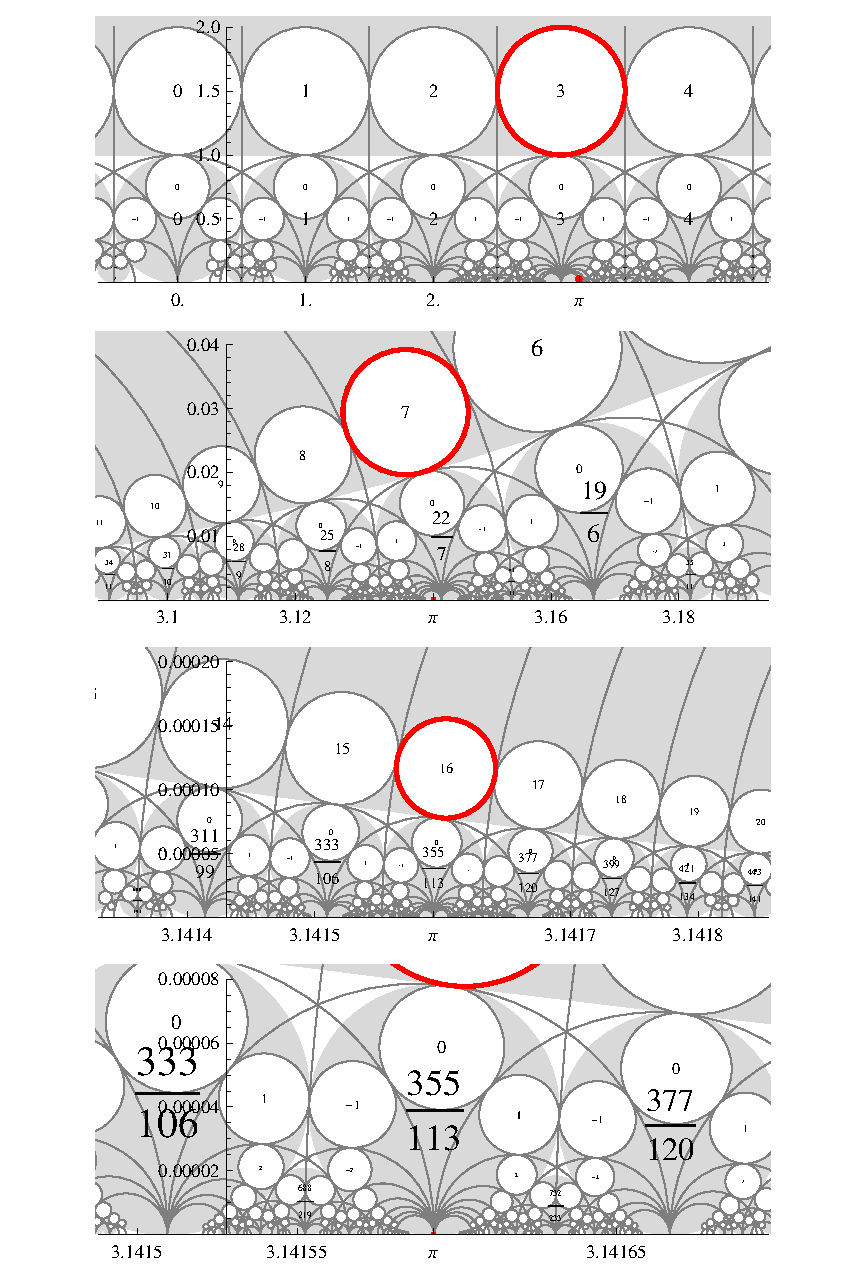
\includegraphics[width=\textwidth]{figures/cont-frac-pi}
\caption{$\pi = \frac{355}{113}$ -- well, almost.}
\label{fig_ContFracPi}
\end{figure}


\todo{19}{The modular group and ford circles}
